\documentclass[25pt, a0paper, portrait, margin=0mm, innermargin=15mm,
     blockverticalspace=15mm,colspace=15mm, subcolspace=8mm]{tikzposter} %Default values for poster format options.



\usepackage{amsthm,amsmath,amsfonts,amssymb}
\usetikzlibrary{arrows.meta, patterns, calc}
\newcommand\NameBlock[1]{\node[fit=(blockbody)(blocktitle),inner sep=5pt] (#1) {};} %to put arrows from/to boxes

\theoremstyle{plain}
\newtheorem{lemma}{Lemma}

\boldmath % make all math bold

 \tikzposterlatexaffectionproofoff %shows small comment on how the poster was made at bottom of poster

\renewcommand*{\familydefault}{\sfdefault}



 % Commands
 \newcommand{\bs}{\textbackslash}   % backslash
 \newcommand{\cmd}[1]{{\bf \color{red}#1}}   % highlights command

 % Title, Author, Institute
 \title{ Look Ma, No Sampling!}
 \author{Colin Fox \& Lennart Golks}
 \institute{University of Otago}
% \titlegraphic{\includegraphics[width=.15\textwidth]{unihorizcmyk-b.jpg}}

\settitle{ \vbox{ \centering
\@titlegraphic\\[\TP@titlegraphictotitledistance] 
 \color{titlefgcolor} \centering {\bfseries \Huge \@title \par} \vspace*{1em} 
{\bf\huge \@author \par} \vspace*{1em} 
{\makebox[0.1em]{\begin{minipage}[b][1em]{39.4cm} \end{minipage}}
\LARGE ISBA BayesComp Singapore 2025
\makebox[0.1em]{\begin{minipage}[b][1em]{40.2cm}  \end{minipage}}
}
}}

 % -- PREDEFINED THEMES ---------------------- %
 % Choose LAYOUT:  Default, Basic, Rays, Simple, Envelope, Wave, Board, Autumn, Desert,
\usetheme{Autumn}

\definecolorpalette{MyColorPalette}{
	 %\definecolor{colorOne}{HTML}{785EF0}
    \definecolor{colorOne}{HTML}{DA5C96}%{D41159}
    %\definecolor{colorThree}{HTML}{CC79A7}
     \definecolor{colorTwo}{HTML}{56B4E9}%{1E88E5}%{1A85FF}
    \definecolor{colorThree}{HTML}{FF8533} %{F88251}
}

%\definecolorpalette{MyColorPalette}{
%    \definecolor{colorOne}{RGB}{0,30,102}
%    \definecolor{colorTwo}{RGB}{162,196,217}
%    \definecolor{colorThree}{RGB}{255,133,41} 
%}

%\definecolorpalette{MyColorPalette}{
%	\definecolor{colorOne}{RGB}{86,180,233} %title color
%	\definecolor{colorTwo}{RGB}{86,180,233} %background color
	%\definecolor{colorTwo}{RGB}{0,158,115} %background color
	%\definecolor{colorThree}{RGB}{213,94,0} %cite box color
%}


%\definecolorpalette{MyColorPalette}{
%	    \definecolor{colorOne}{RGB}{0,30,102}
%	   \definecolor{colorTwo}{RGB}{162,196,217}
%	    \definecolor{colorThree}{RGB}{255,133,41} 
%	}

\usecolorstyle[colorPalette=MyColorPalette]{Germany}
% COLORPALETTE: Default, BlueGrayOrange, GreenGrayViolet, PurpleGrayBlue, BrownBlueOrange.
% COLORSTYLE: Default, Australia, Britain, Sweden, Spain, Russia, Denmark, Germany

\newcommand{\dd}{\mathrm{d}}
\newcommand{\bbR}{\mathbb{R}}
\newcommand{\tsfrac}[2]{{\textstyle \frac{#1}{#2}}}
\newcommand{\twobyone}[2]{\begin{array}{c} #1 \\ #2 \end{array}}
\newcommand{\twobytwo}[4]{\begin{array}{cc} #1 & #2 \\ #3 & #4 \end{array}}

\newcommand{\E}{\operatorname{E}}

\usepackage{graphicx}
\usepackage{amsmath, bm}
\usepackage{pgfplots}
\pgfplotsset{compat=1.18}
\usetikzlibrary{decorations.pathreplacing,calligraphy}
\usetikzlibrary{positioning}
\usetikzlibrary{positioning,shapes.symbols,fit}
\tikzset{
	roundnode2/.style={circle, draw=green!50!blue, very thick, minimum size=9mm},
	roundnode/.style={circle, draw=green!50!blue, fill=green!60!blue, very thick, minimum size=7mm},
	rectnode/.style={rectangle, draw=green!50!blue, very thick, minimum size=8.5mm},
	mydotted/.style = {dash pattern=on 6.1pt off 7pt, line width = 3pt},
	myline/.style = {line width = 3pt}
}


\begin{document}
\maketitle



\begin{columns}
\column{1}
\block{Tired of waiting for your MCMC to run? No problem, just skip the MCMC and evaluate expectations using tensor train function representation and numerical integration.\\[-1.5em]}{}
\end{columns}
\NameBlock{firstcol}

\begin{columns}
\column{.33}
\block{Bayesian Formulation  }{\vspace*{-2ex}
\tikzstyle{unknown}=[circle,draw=blue!100,ultra thick,minimum size=2.5em] %!nn appears to be how opaque as percentage
\tikzstyle{measured}=[rectangle,draw=blue!100,ultra thick,minimum size=2.5em]
\begin{tikzpicture}%[node distance=4em]
  \node[measured] (data) {$y$};
  \node[unknown] (x)             [above of=data, node distance=4em]    {$x$};
  \node[unknown] (theta)         [above of=x, node distance=4em]          {$\theta$};
  \draw [-{Latex[length=6mm]},ultra thick] (x) to (data);
  \draw [-{Latex[length=6mm]},ultra thick] (theta) to (x);

  %\node (hyper) [right of=theta, node distance=6em,inner sep=0pt, align=left]  {Hyperparameters: Hyper-prior: $[\theta]$};
  \node[right of=theta, node distance=2em, inner sep=0pt, align=left, anchor=west] (hyper) {Hyperparameters: Hyper-prior: $[\theta]$};
  \node[right of=x, node distance=2em, inner sep=0pt, align=left, anchor=west] (hyper) {Latent field: Representation and prior $[x|\theta]$};
  %\node (prior) [right of=x, node distance=5em,inner sep=0pt]  {Prior model: representation and $[x|\theta]$};
  %\node (obs) [right of=data, node distance=6em,inner sep=0pt]  {Observed data: Likelihood: $[y|x]$};
  \node[right of=data, node distance=2em, inner sep=0pt, align=left, anchor=west] (obs) {Observed data: Likelihood: $[y|x]$};
\end{tikzpicture}

}
\NameBlock{bayes}
\column{.33}

\block{Posterior Inference}{\vspace*{-2ex}
 The focus of inference is the posterior distribution:
%
\[ [x,\theta|y] = \frac{[y|x]\,[x|\theta]\,[\theta]}{[y]} \]
We assume the normalizing constant $[y]$ is finite.

We wish to compute expectations:
\coloredbox{
\[ \E_{x,\theta|y}[f(x)] = \int f(x) [x,\theta|y]\,\dd x\,\dd\theta \]
}
%\centerline{`Keep you eyes on the prize'}
}
\NameBlock{expect}





% \note[targetoffsetx=1cm, targetoffsety=-1.5cm,rotate=2,angle=270,radius=8cm,width=.5\textwidth,innersep=.4cm]{
% {\large A jaunty note.}
% }

\column{.33}

\block{This Notation}{
We learned this notation from Alan Gelfand:\\Read $[a]$ as ``the distribution over $a$'', and $[a|b]$ as ``the distribution over $a$ given $b$''. We will abuse this notation to also denote the density function.
}
\NameBlock{notation}
\end{columns}
\NameBlock{seccol}


\begin{columns}
\column{0.5}
\block{Quadrature and the Law of Total Expectation}{\vspace*{-2ex}
% Factorise posterior density into the full conditional for $x$ and the marginal posterior over $\theta$.
% \[ [x,\theta|y] = [x|\theta,y]\,[\theta|y] \]
 The posterior expectation of any function $h(x)$ may be written
\[
\text{E}_{x,\theta |y}\left[ h\left(x \right) \right] = \text{E}_{\theta |y}\left[ \text{E}_{x |\theta,y}\left[ h\left(x \right) \right] \right]
\]
% \begin{itemize}
%  \item Hyperparameters $\theta$ are typically low dimensional
%  \item Latent process $x$ can be high-dimensional
% \end{itemize}
%
We compute the outer expectation by quadrature (see next panel). When the inner expectation is cheap to calculate, %(e.g. mean of GMRF by linear algebra)
evaluating $\text{E}_{x,\theta |y}\left[ h\right]$  requires \textbf{no MCMC}.
% \coloredbox{
% See: C.~Fox and R.~A. Norton.
% \newblock Fast sampling in a linear-{G}aussian inverse problem.
% \newblock {\em SIAM/ASA Journal on Uncertainty Quantification},
%   4(1):1191--1218, 2016.
% }
}
\NameBlock{total}


\block{Marginal Posterior over Hyperparameters $[\theta|y]$ }{\vspace*{-2ex}
\[ [\theta|y]=\int_X [x,\theta|y]\,\dd x \tikz[remember picture,baseline=(B.base)] \node (B) at (0,0) {};\]
%Avoid calculating this integral  over the high-dimensional latent field $x$. \\
A cheap algebraic calculation is available when the full conditional for $x$
\[ [x | \theta, y] = \frac{[ y | x]\,[ x | \theta ]}{[y|\theta]} \]
has known form. Then the normalising constant $[y|\theta]$ has known $\theta$ dependence, and %hence one can evaluate the marginal posterior over $\theta$
\[ [\theta | y] \propto [ y | \theta]\,[\theta]. \]
\coloredbox{R.~A. Norton, J.~A. Christen, and C.~Fox.
\newblock Sampling hyperparameters in hierarchical models: improving on {Gibbs}
  for high-dimensional latent fields and large datasets.
\newblock {\em Communications in Statistics - Simulation and Computation},
  47(9):2639--2655, 2018.
}

}
\note[targetoffsetx=5.5cm,targetoffsety=6.5cm,innersep=.4cm,angle=7,connection,radius=8cm,width=10cm]{Avoid calculating this integral  over high-dimensional latent field $x$.}

\block{Tensor Train Representation of $[\theta|y]$}{
\centering
A surface rendering of a density in TT format \\ TT formula
\begin{minipage}[b]{0.7\columnwidth}
	\begin{flushleft} \input{TTSchem.pdf_tex}\end{flushleft}
\end{minipage} \hfill %\hspace{1cm}
\begin{minipage}[b]{0.3\columnwidth}
			\vspace{-5cm}
		\begin{flushright} 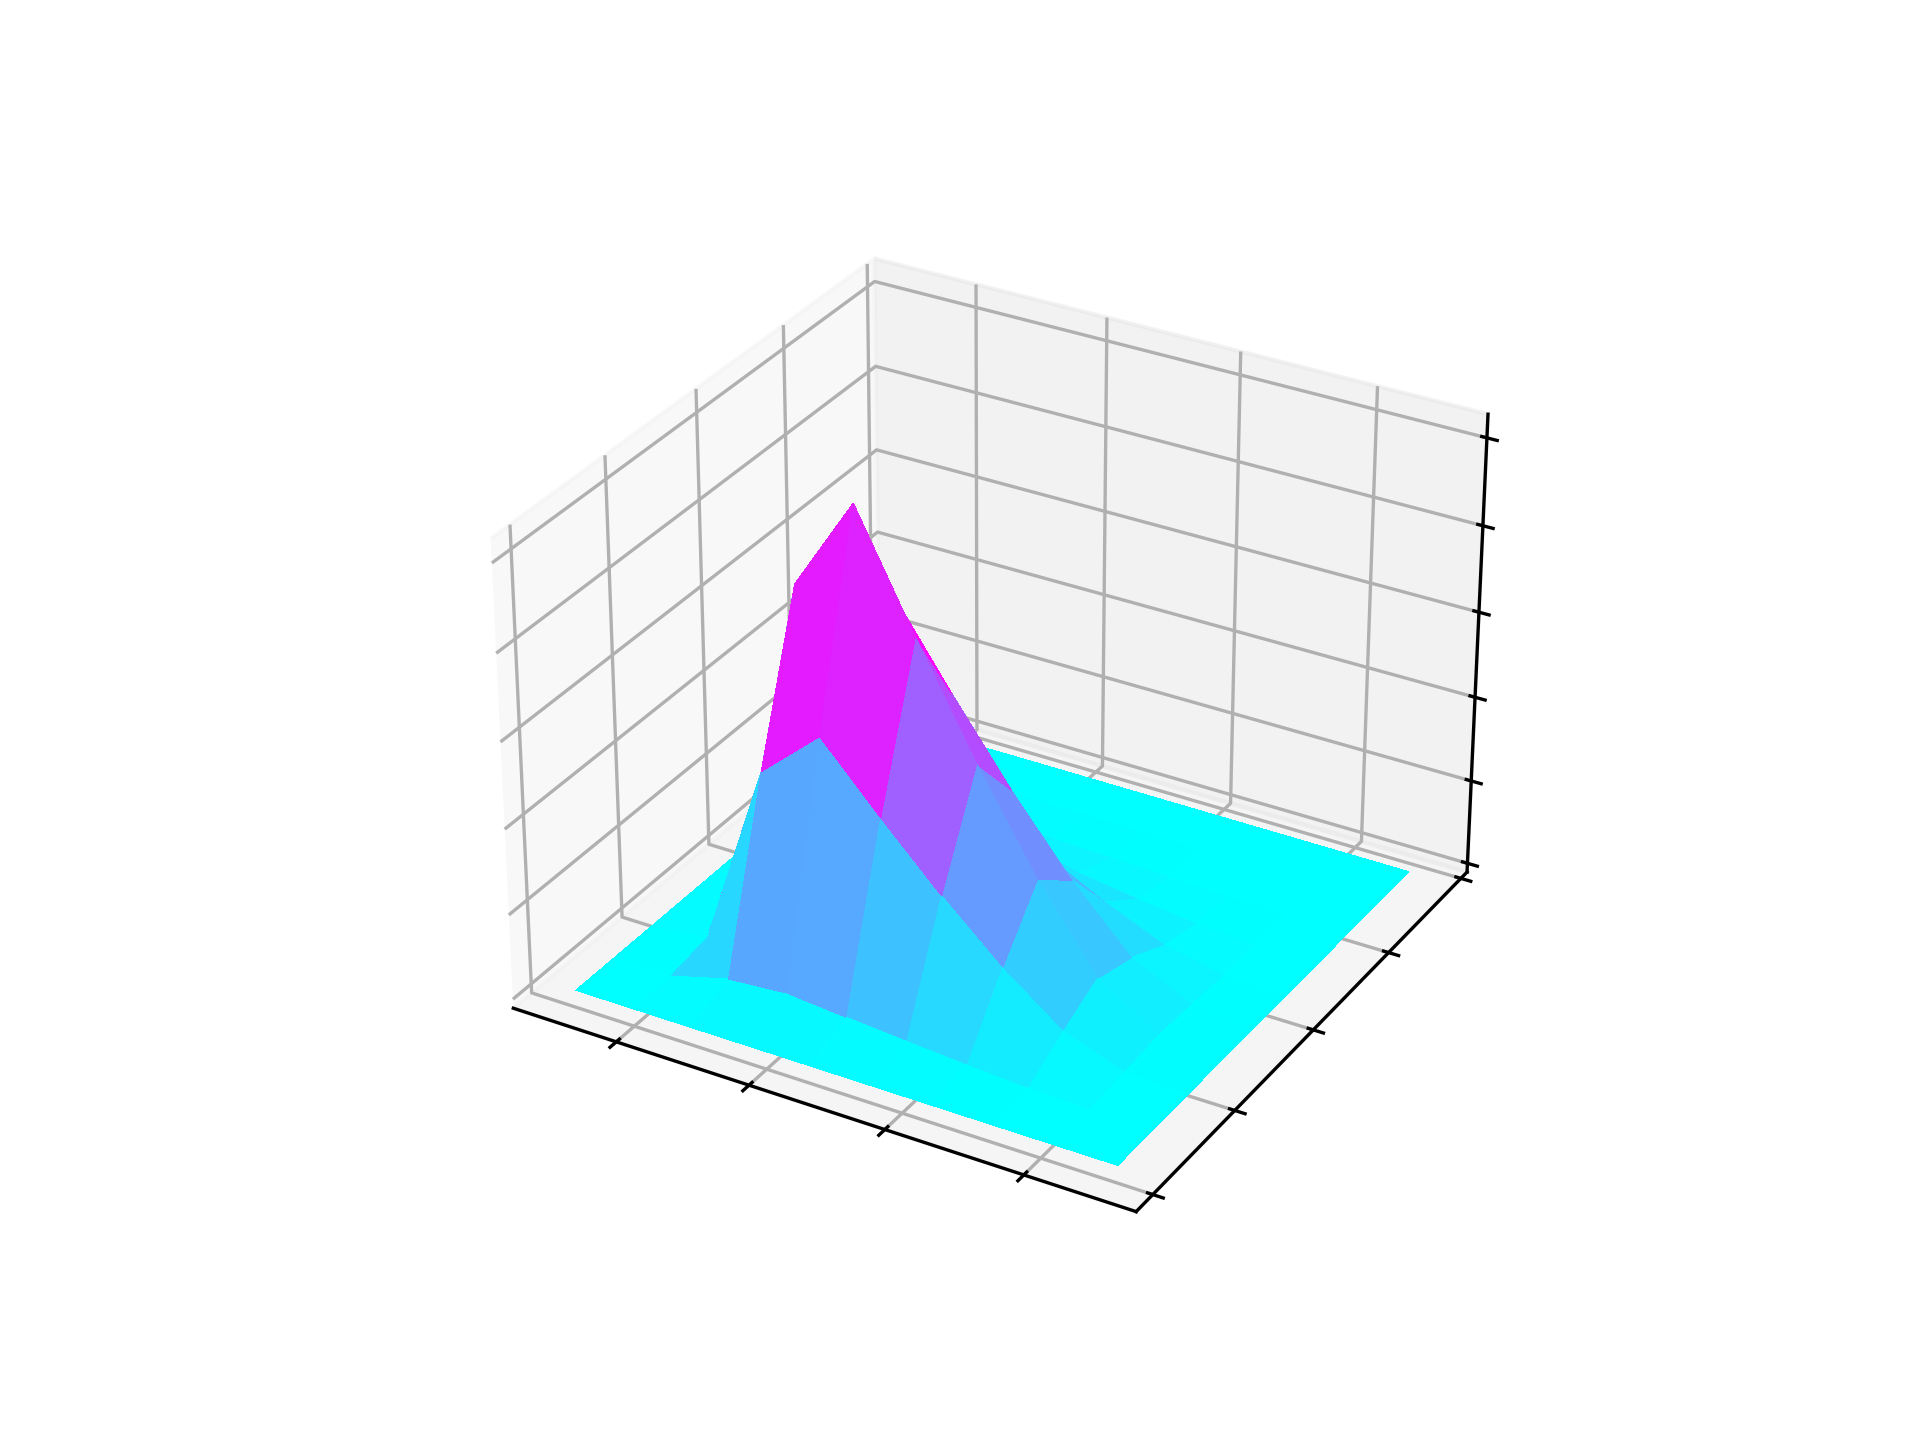
\includegraphics[]{PosterMargTT.png}\end{flushright}
%\centering 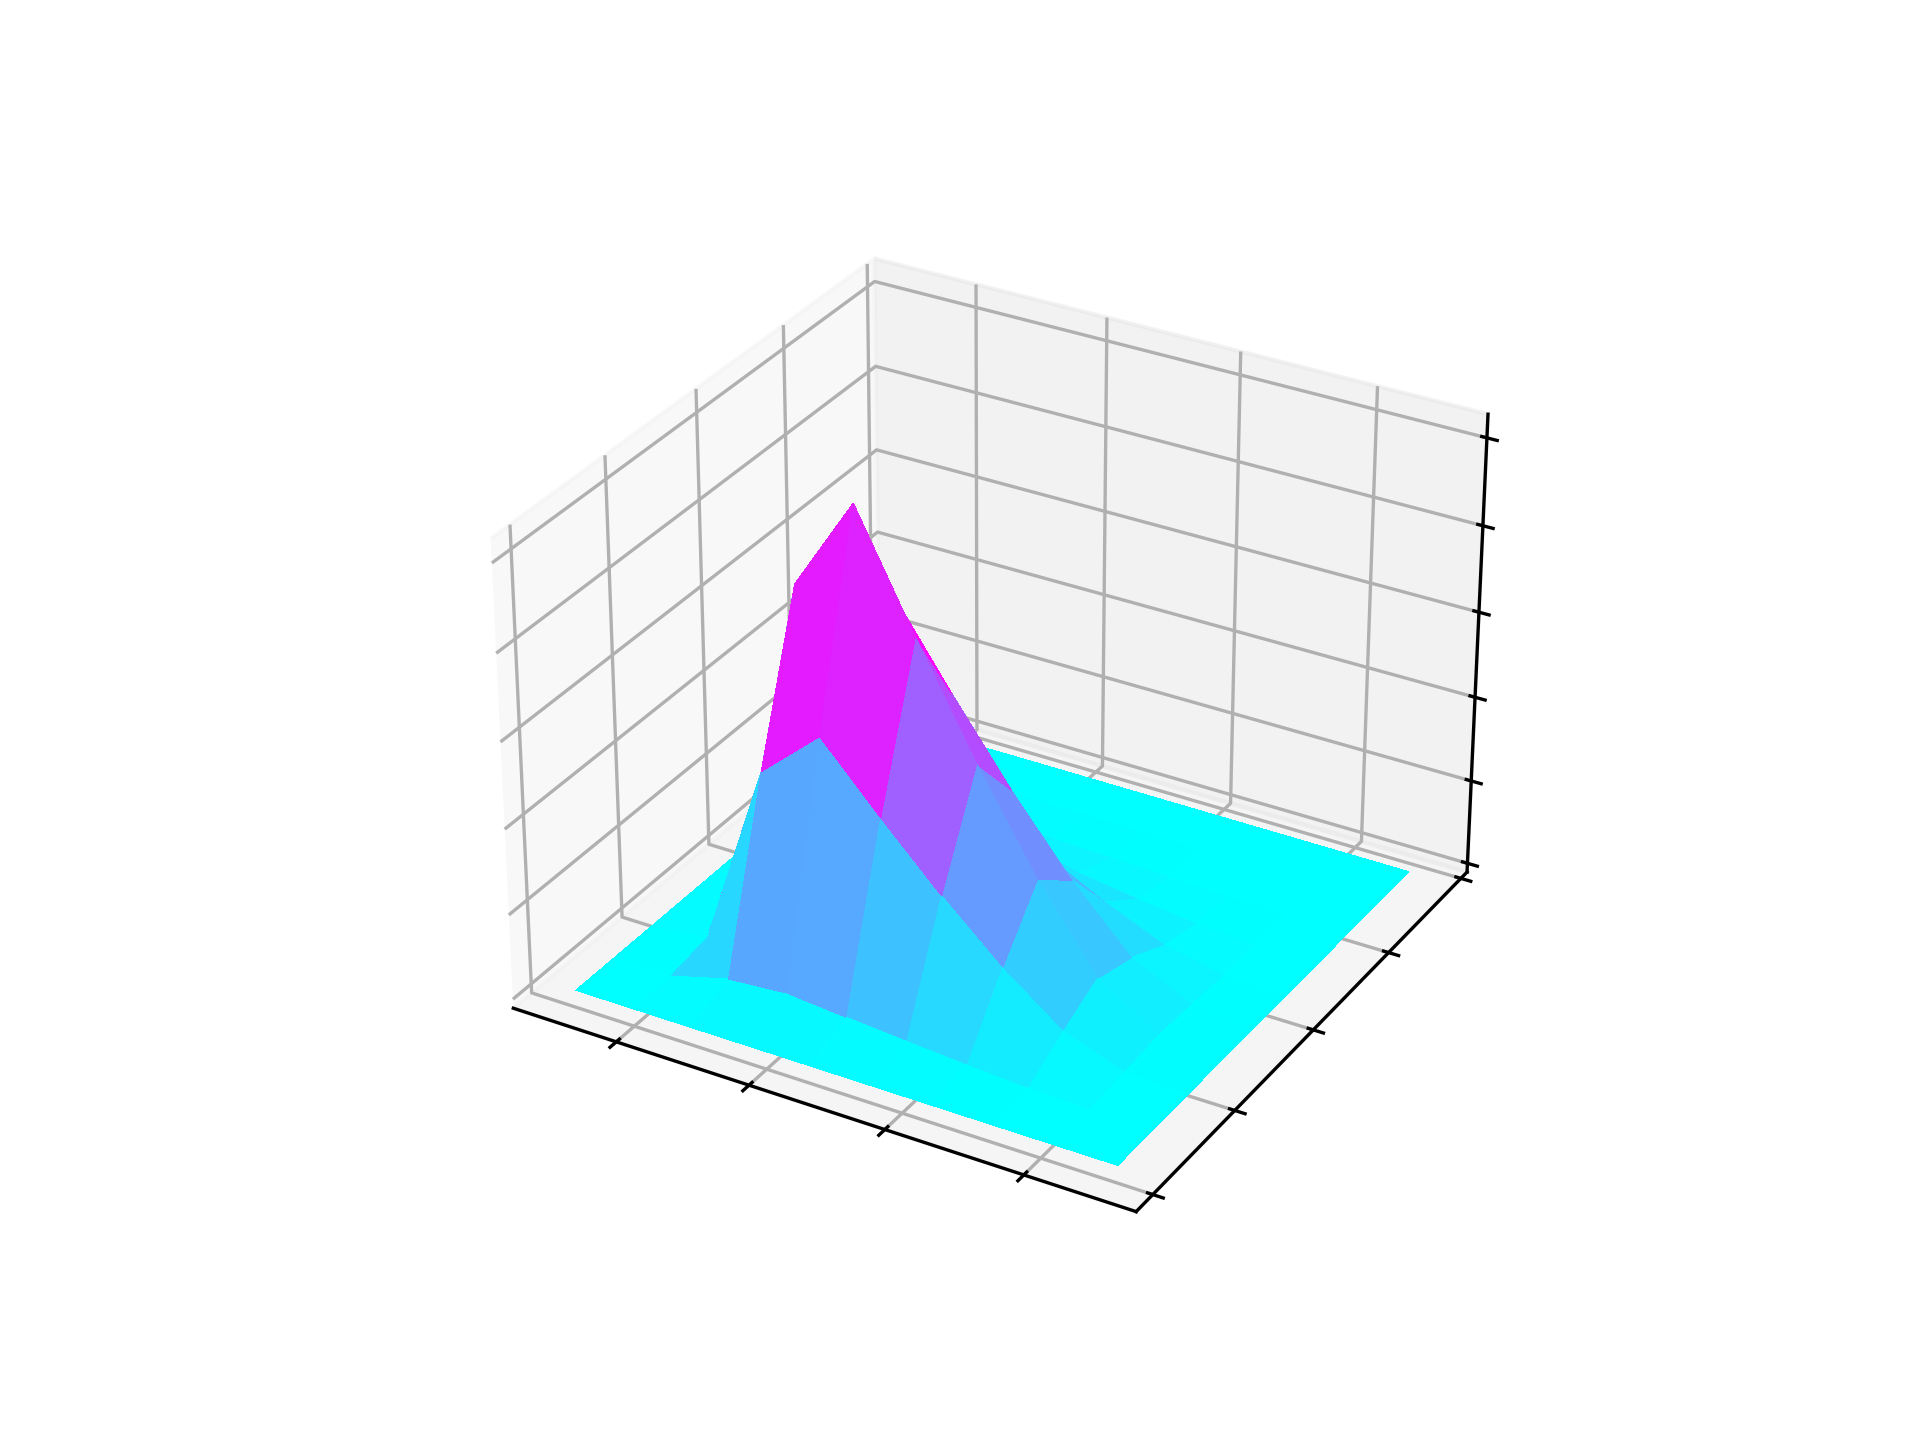
\includegraphics[]{PosterMargTT.png}
\end{minipage}	
%After computing the coefficient tensors $\bm{B}_{\text{pre}, k+1}$ as in Prop.~\ref{prob:ForMarg} and $\bm{B}_{k+1}$ from Prop.~\ref{prob:backMarg}, the marginal PDF of $k$-th dimension can be expressed as
\resizebox{.45\columnwidth}{!}{
$f_{X_k}(x_k) = \frac{1}{z} \left(\gamma^{\prime} \prod_{i=1}^{k-1} \lambda_i(X_i) \prod_{i=k+1}^{d} \lambda_i(X_i) + \sum_{l_{k-1}=1}^{r_{k-1}} \sum_{l_k=1}^{r_k} \left(\sum_{i=1}^{n} \phi^{(i)}_k(x_k) \bm{D}_k[l_{k-1},i, l_k] \right)^2 \right) \lambda_k(x_k)$}
%where $\bm{D}_k \in \mathbb{R}^{r_{k-1} \times n \times r_k}$ and $\bm{R}_{\text{pre},k-1}\in \mathbb{R}^{r_{k-1} \times r_{k-1}}$ and $\bm{B}_k \in \mathbb{R}^{r_{k-1} \times n \times r_k}$
%\begin{equation}
%	\bm{D}_k[l_{k-1},i,l_k] = \sum_{\alpha_{k-1}=1}^{r_{k-1}}  \bm{R}_{\text{pre},k-1}[l_{k-1}, \alpha_{k-1}] \bm{B}_k[\alpha_{k-1}, i, l_k].
%\end{equation}

\coloredbox{S.~Dolgov, K.~Anaya-Izquierdo, C.~Fox, and R.~Scheichl.
\newblock Approximation and sampling of multivariate probability distributions
  in the tensor train decomposition.
\newblock {\em Statistics and Computing}, 30(3):603--625, 2020. }
}

\column{0.5}
\block{Monte Carlo Integration}{{~}\\[-3em]
\begin{align*}
 \E_{x,\theta|y}[f(x)] %&= \int f(x) \pi(x,\theta|y)\,\dd x\dd\theta\\
                     &\approx \frac{1}{N}\sum_{i=1}^N f(x_i)
\end{align*}
where %$(x_i,\theta_i)\sim \pi(x,\theta|y)$, or more generally
$\left\{(x_i,\theta_i)\right\}$ is ergodic for $[x,\theta|y]$.
\coloredbox{
\begin{quotation}
 ``Monte Carlo is an extremely bad method; it should be used only when all alternative methods are worse.'' (Alan Sokal)
\end{quotation}
}
}
\NameBlock{carlo}

\block{Markov chain Monte Carlo}{
A representative MCMC scheme is the block Gibbs sampler %that updates  $(x,\theta)$ to $(x',\theta')$ by alternating drawing from full conditionals
\begin{itemize}
 \item Draw $\theta'\sim [\theta|x]$
 \item Draw $x' \sim [x|\theta',y]$
\end{itemize}
simulating a transition kernel that targets the posterior $[x,\theta|y]$.\\
%\centerline{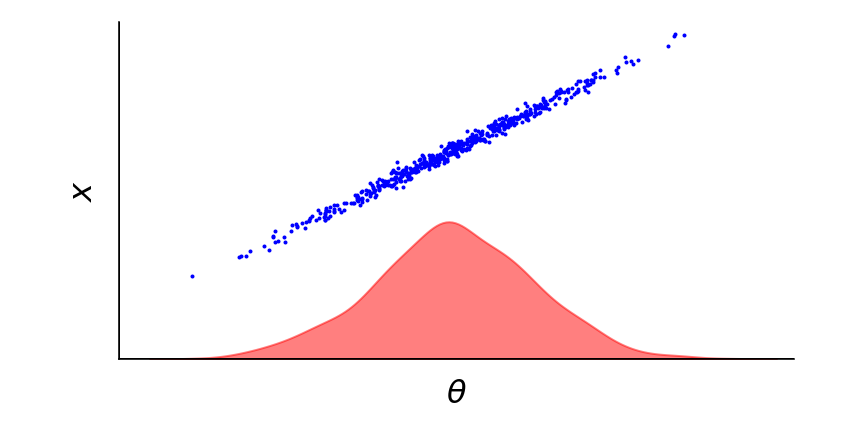
\includegraphics[]{scatterplotmarginal.png}}
Narrow scatter plot shows why this is slow --
\coloredbox{Better is to move in the marginal posterior over hyperparameters $[\theta|y]$\\
            H.~Rue and L.~Held.
\newblock {\em Gaussian {M}arkov random fields : {T}heory and applications}.
\newblock Chapman Hall, New York, 2005.}
}

\block{Independent Posterior Sampling (MTC) }{
% Factorise posterior density into the full conditional for $x$ and the marginal posterior over $\theta$.
% \[ [x,\theta|y] = [x|\theta,y]\,[\theta|y] \]
If the inner expectation is not available exactly, draw \emph{independent} posterior samples by:
\centerline{Use TT representation to sample $\theta'\stackrel{\text{iid}}{\sim} [\theta|y]$ then $x'\sim [x|\theta',y]$}

% % \begin{lemma}
% %\label{lem:mtc}
% \textbf{Lemma} Sampling $\theta'\sim [\theta|y]$ then $x'\sim [x|\theta',y]$
% generates a sample from the posterior distribution, i.e.,
% \[ \left(x' ,\theta'\right) \sim [x,\theta|y]. \]
% % \end{lemma}

\coloredbox{
C.~Fox and R.~A. Norton.
\newblock Fast sampling in a linear-{G}aussian inverse problem.
\newblock {\em SIAM/ASA Journal on Uncertainty Quantification},
  4(1):1191--1218, 2016.
}
%
}

\end{columns}

\begin{columns}
\column{.45}

\block{Inverse Problem of Recovering Ozone Profile }{
	%\column{.49}
	\centering

	\begin{minipage}[b]{0.45\linewidth}

	\input{LIMBPoster.pdf_tex}
		\resizebox{\columnwidth}{!}{
		$y_j =   \int_{\Gamma_j}  B(\nu,T) k(\nu, T)   \frac{p(T)}{k_{\text{B}} T(r)}  x(r)  \tau(r) \text{d}r + \eta_j \,$}\\
		\resizebox{0.9\columnwidth}{!}{
	$\tau(r) = \exp{ \Bigl\{ - \int^{r}_{r_\text{obs}}  k(\nu, T)   \frac{p(T)}{k_B T(r^{\prime})}  x(r^{\prime}) \text{d}r^{\prime} \Bigr\} }  $ }\\
	\\
		\resizebox{0.9\columnwidth}{!}{
	$\bm{y} = \bm{M} \bm{A} \bm{x} + \bm{\eta} $ }
\vspace{1cm}
\end{minipage}\hfill
\begin{minipage}[b]{0.54\linewidth}
		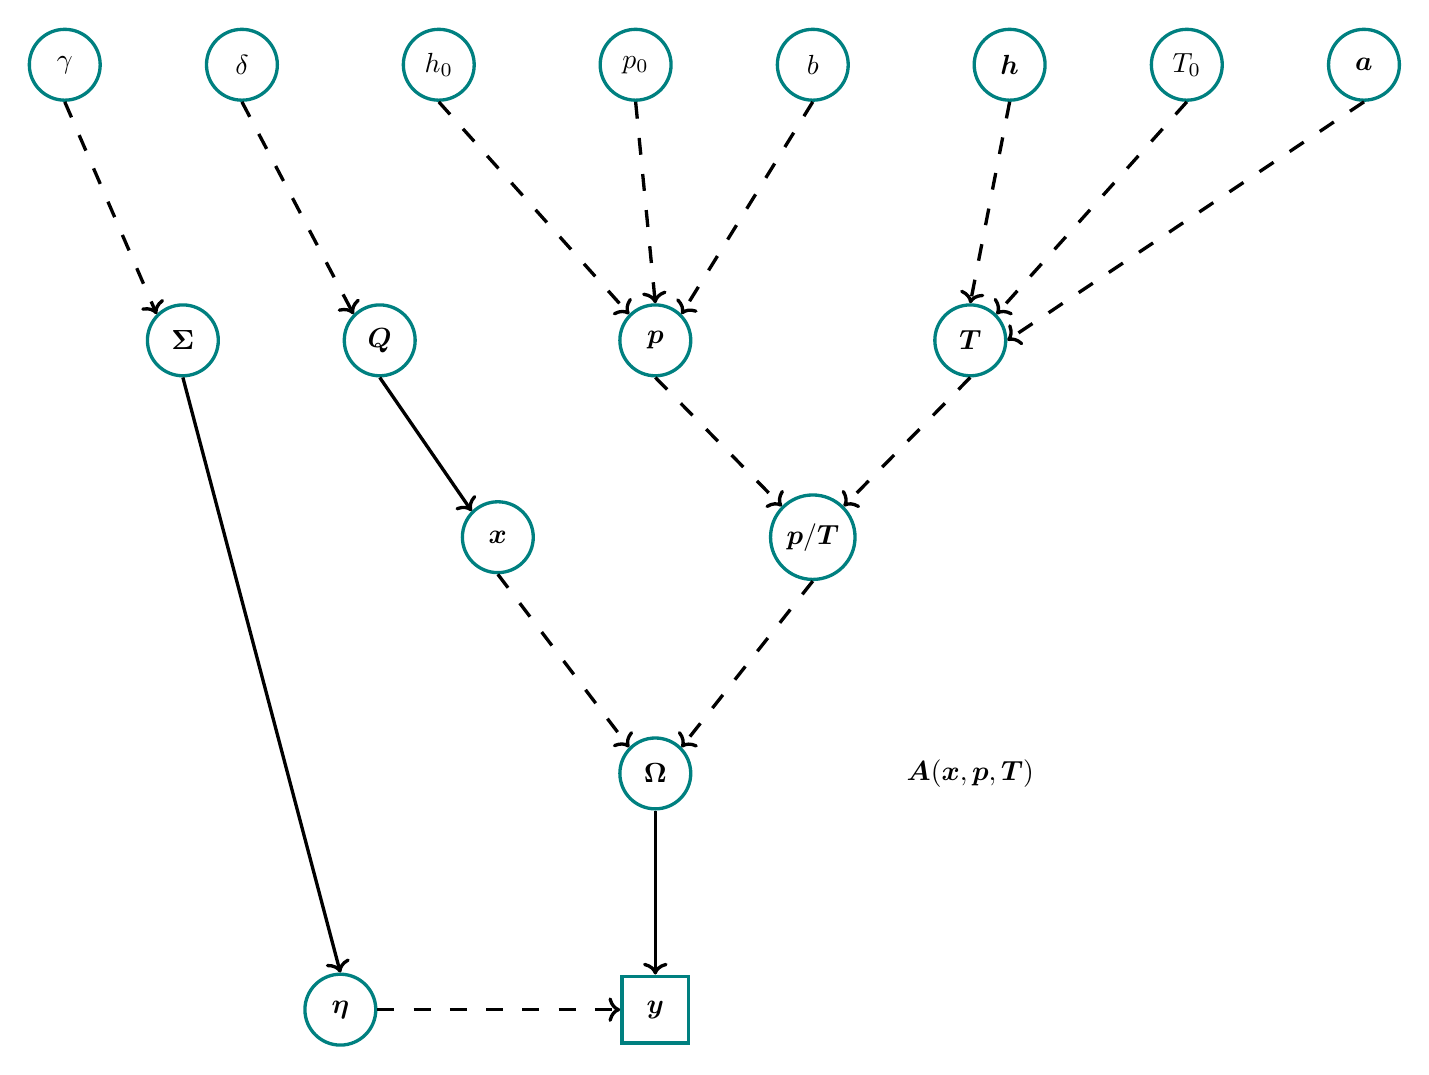
\begin{tikzpicture}
		\node[roundnode2] at (-4.5,6.5) (Q)     {$\bm{Q}$};
		\node[roundnode2] at (-3,4) (x)     {$\bm{x}$};
		\node[align=center] at (3,1) (A)    {$\bm{A}(\bm{x},\bm{p},\bm{T})$};
		\node[roundnode2] at (-1,1) (u)    {$\bm{\Omega}$};
		\node[rectnode] at (-1,-2) (y)    {$\bm{y}$};
		\node[roundnode2] at (-5,-2) (e)    {$\bm{\eta}$};
		\node[roundnode2] at (-7,6.5) (S)    {$\bm{\Sigma}$};
		\node[roundnode2] at (-8.5,10) (s)    {$\gamma$};
		\node[roundnode2] at (-6.25,10) (d)    {$\delta$};
		\node[roundnode2] at (3,6.5) (t)     {$\bm{T}$};
		\node[roundnode2] at (-1,6.5) (p)     {$\bm{p}$};
		\node[roundnode2] at (1,4) (pt)     {$\bm{p}/\bm{T}$};
		\node[roundnode2] at (1,10) (b1)    {$b$};
		%\node[roundnode2] at (1,8) (b2)    {$b_2$};
		\node[roundnode2] at (-3.75,10) (h1)    {$h_{0}$};
		\node[roundnode2] at (-1.25,10) (p0)    {$p_0$};
		\node[roundnode2] at (3.5,10) (ht)    {$\bm{h}$};
		\node[roundnode2] at (5.75,10) (ct)    {$T_0$};
		\node[roundnode2] at (8,10) (at)    {$\bm{a}$};
		
		%Lines
		\draw[->, very thick] (S.south) -- (e.north);
		\draw[->, mydotted, very thick] (s.south) -- (S.north west);
		\draw[->, very thick] (u.south) -- (y.north);
		%\draw[->, mydotted, very thick] (A.south) -- (u.north);
		\draw[->, mydotted,  very thick] (x.south) -- (u.north west);
		\draw[->, mydotted, very thick] (p.south) -- (pt.north west);
		\draw[->, mydotted, very thick] (t.south) -- (pt.north east);
		\draw[->, mydotted, very thick] (pt.south) -- (u.north east);
		\draw[->, mydotted, very thick] (h1.south) -- (p.north west);
		\draw[->, mydotted, very thick] (p0.south) -- (p.north);
		\draw[->, mydotted, very thick] (b1.south) -- (p.north east); 
		%\draw[->, very thick] (b2.south) -- (p.east); 
		\draw[->, mydotted, very thick] (d.south) -- (Q.north west); 
		\draw[->, mydotted, very thick] (e.east) -- (y.west); 
		
		\draw[->, very thick] (Q.south) -- (x.north west); 
		\draw[->, mydotted, very thick] (ht.south) -- (t.north);
		\draw[->, mydotted, very thick] (ct.south) -- (t.north east);
		\draw[->, mydotted, very thick] (at.south) -- (t.east);
		%\node[align=center] at (0.25,3.95) (f3) {$\approx \bm{M A}_L$};
	\end{tikzpicture} 
\end{minipage}
}


\column{.55}
\block{Posterior Expectation by TT  and Affine Representations}{Picture of posterior inference, or timings, or some output summaries -- perhaps a box below with some snappy summary or conclusions
	\begin{minipage}{0.2\linewidth}
			\begin{flushleft} 
		\begin{tikzpicture}
			\foreach \X [count=\Z]in {0,1,2,3,4}
			{\node[opacity=0.8] at (-\Z*1.25,0,\Z*1.75) {\includegraphics[]{PHdPTPost\X}};}
		\end{tikzpicture}
			\end{flushleft} 
\end{minipage}
\begin{minipage}{0.2\linewidth}
\begin{itemize}
	\item 
\end{itemize}
\end{minipage}

}
\end{columns}


%\draw [black, myline,rounded corners ] ($(Bayes) + (-13.5,8) $)  -- ($(Bayes) + (68.5,8) $)  -- ($(Bayes) + (68.5,-8) $) --($(Bayes) + (-13.5,-8) $) --  cycle;
\draw [black, myline,rounded corners ] ($(bayes.north west) + (-0.5,0.5)$ )  -- ($(notation.north east) +  (0.5,0.5)$ )  -- ($(notation.south east) +  (0.5,-5.25)$ )  -- ($(bayes.south west) + (-0.5,-0.5)$ )  --  cycle;


\draw [black, myline,rounded corners ] (firstcol.north west)  -- (firstcol.north east)  -- (firstcol.south east)   -- (firstcol.south west)  --  cycle;

\node[above = 1] at (expect) {\huge try blblbl};

%\node (total.130) {some text};
\node[align = left] at (total.130) {\textcolor{red}{\huge DO THIS}};
\node[align = right] at (carlo.40) {\textcolor{red}{\huge DON'T DO THIS}};

\begin{scope}[transparency group, opacity=0.5]
\draw [-latex, orange, line width=15mm] (expect.south west) ++(1,1.5) to (total.85);
\draw[-latex, orange, line width=15mm] (expect.south east) ++(-.7,1.5) -- (carlo.100); % 100 is angle
\end{scope}






\end{document}

\endinput
%%
